\documentclass[10pt,letterpaper]{article}
\usepackage[utf8]{inputenc}
\usepackage{amsmath}
\DeclareMathOperator{\sign}{sgn}
\usepackage{amsfonts}
\usepackage{amssymb}
\usepackage[margin=0.5in]{geometry}
\usepackage{graphicx}
\usepackage{sidecap}
\usepackage{float}

\usepackage[font=small,labelfont=bf]{caption}


\title{\vspace{-4ex}Regression and SVM\vspace{-3.5ex}}
\begin{document}
\newgeometry{top=0.75in,left=0.75in,right=0.75in,bottom=1.25in}
\maketitle
\vspace{-0.5em}
\begin{abstract}
Previously, we discussed various methods for polynomial regression and minimizing error in our objective function, and explored famous examples, namely ridge regression and other norms (i.e. LAD for the L1 norm). Here, we will extend those concepts to a few classification problems, through logistic regression (a natural adaptation of the polynomial regression we've been doing) and then more formally through the concept of support vector machines (SVMs).
\end{abstract}

\section{Logistic Regression}
In past discussions, we've often encountered the objective function of our MLE estimate, or of some other estimate that we've established for some parameter $\theta$ that we'd like to minimize so as to minimize the value of our error function. This is called \textbf{regression}. Here we will discuss \textbf{logistic regression}, which involves fitting the data to a curve of the form
$$\sigma(x) = \frac{1}{1+e^{-x}}$$
This is known as the \textbf{sigmoid} function, and it's often used when the data we would like to fit is well-modeled as a classification problem (with labels +1 and -1). Given $d$-dimensional data $x^{(1)}, x^{(2)}, ... , x^{(n)}$ and corresponding scalar labels $y^{(1)}, y^{(2)}, ... , y^{(n)}$, we can define our LR objection function as:
$$\text{NLL}(w) = \sum_{i=0}^n\log(1+e^{-y^{(i)}(x^{(i)}\cdot w+w_0)})$$
given the parameters $w, w_0$. To reduce overfitting, we can apply an $L2$ regularization term to our equation, as in ridge regression. As a result, we are simply minimizing
$$E_{LR}(w) = \text{NLL}(w)+\lambda w^\intercal w$$
so that
$$w^* = \text{argmin}_w \left[\sum_{i=0}^n\log(1+e^{-y^{(i)}(x^{(i)}\cdot w+w_0)}) + \lambda w^\intercal w\right]$$

We can estimate $w$ numerically using stochastic gradient descent; if we let $\lambda = 0$, then we have no regularization and we end up with this data, as well as figures 1-8:
\begin{table}[h]
\centering
\caption{$\lambda=0$ (step = .001, threshold = .008)}
\begin{tabular}{r|cc|cc|cc|cc}
   & \multicolumn{2}{|c}{\texttt{stdev1}} & \multicolumn{2}{|c}{\texttt{stdev2}} & \multicolumn{2}{|c}{\texttt{stdev4}} & \multicolumn{2}{|c}{\texttt{data\_nonsep}}\\
$w_{init}$& \#it         & Loss        & \#it   & Loss &
\#it   & Loss           & \#it        & Loss      \\\hline
$[1, 1, 1]$  & 255           &    0        & 91      & 0.09             & 49    & 0.32           & 37            & 0.48        \\
$[4, 4, 4]$  & 466           & 0         & 259     & 0.12             & 91      & 0.36            & 64           & 0.44      \\
$[1, 10, 0]$ & 408           &  0         & 354      & 0.11              &  39     & 0.33           & 32            & 0.53      \\
$[-5, -5, -5]$ & 299         &  0        & 199     & 0.1               &  89     & 0.33            & 73           & 0.49    
\end{tabular}
\end{table}

However, if we vary $\lambda$, then we obtain more stable solutions with respect to $w$, and the solutions are more constant regardless of the starting paramters. Figure 9-12 show the decision bounday for $\lambda = 20$.
\begin{figure}[!htb]
\minipage{0.25\textwidth}
  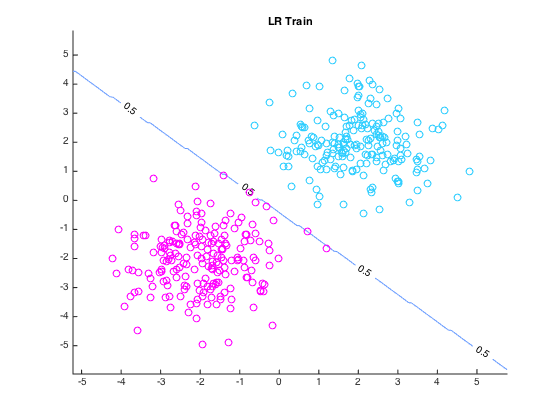
\includegraphics[width=\linewidth]{figures/sd1t0.png}
  \caption{\texttt{stdev = 1}}\label{fig:gradDifQ}
\endminipage\hfill
\minipage{0.25\textwidth}
  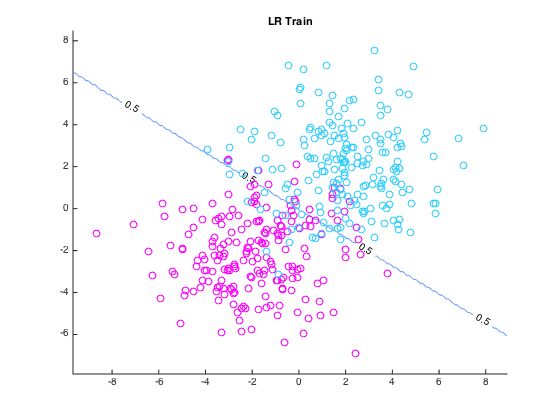
\includegraphics[width=\linewidth]{figures/sd2t0.png}
  \caption{\texttt{stdev = 2}}\label{fig:gradDifN}
\endminipage\hfill
\minipage{0.25\textwidth}
  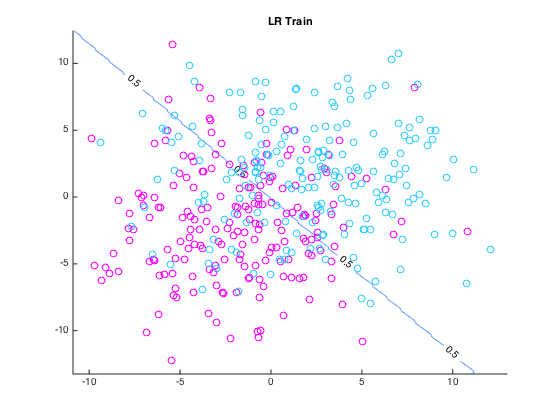
\includegraphics[width=\linewidth]{figures/sd4t0.png}
  \caption{\texttt{stdev = 4}}\label{fig:gradDifS}
\endminipage\hfill
\minipage{0.25\textwidth}
  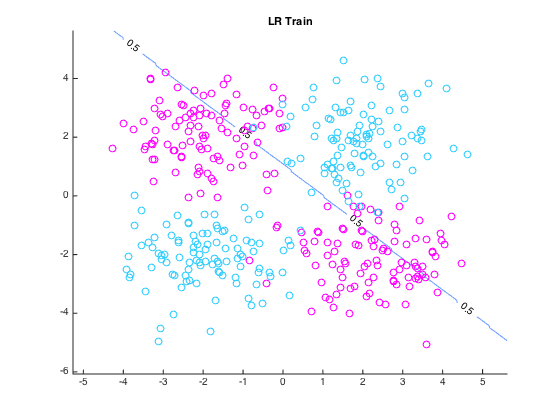
\includegraphics[width=\linewidth]{figures/sdnt0.png}
  \caption{\texttt{unseparable}}\label{fig:gradDifS}
\endminipage
\end{figure}
\begin{figure}[!htb]
\minipage{0.25\textwidth}
  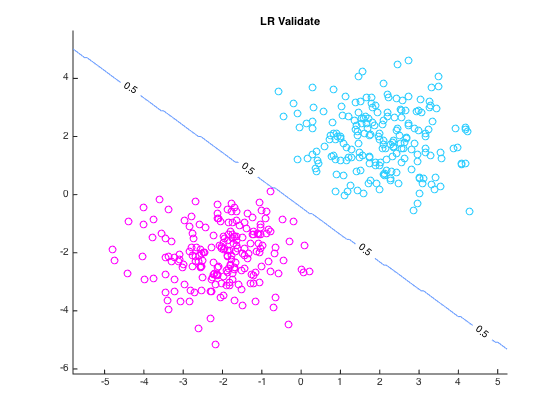
\includegraphics[width=\linewidth]{figures/sd1v0.png}
  \caption{\texttt{stdev = 1}}\label{fig:gradDifQ}
\endminipage\hfill
\minipage{0.25\textwidth}
  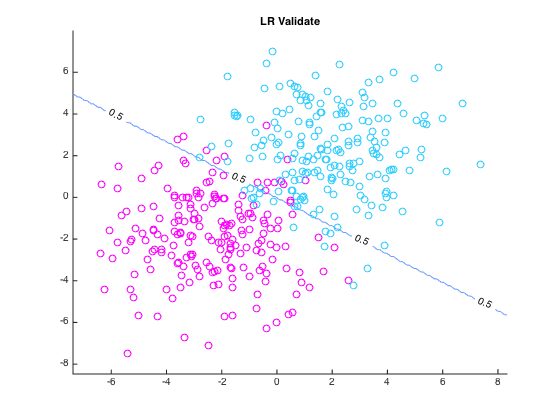
\includegraphics[width=\linewidth]{figures/sd2v0.png}
  \caption{\texttt{stdev = 2}}\label{fig:gradDifN}
\endminipage\hfill
\minipage{0.25\textwidth}
  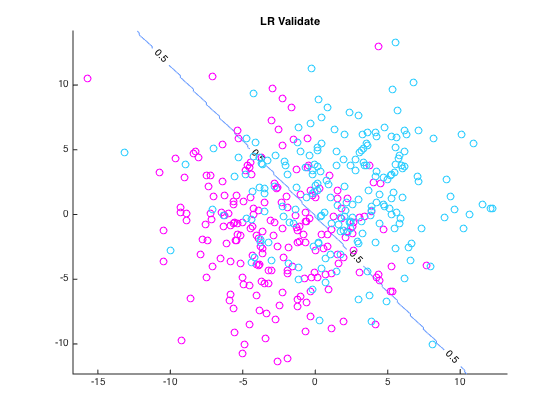
\includegraphics[width=\linewidth]{figures/sd4v0.png}
  \caption{\texttt{stdev = 4}}\label{fig:gradDifS}
\endminipage\hfill
\minipage{0.25\textwidth}
  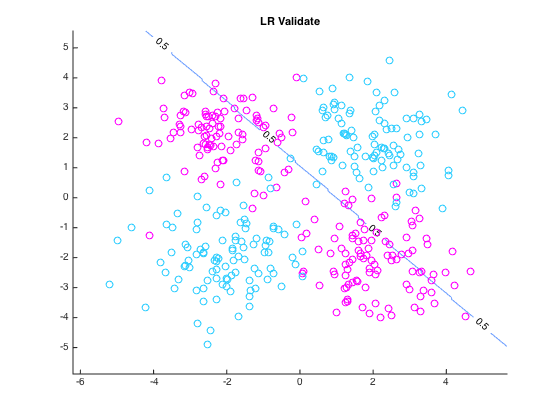
\includegraphics[width=\linewidth]{figures/sdnv0.png}
  \caption{\texttt{unseparable}}\label{fig:gradDifS}
\endminipage

\end{figure}


\begin{figure}[!htb]
\minipage{0.25\textwidth}
  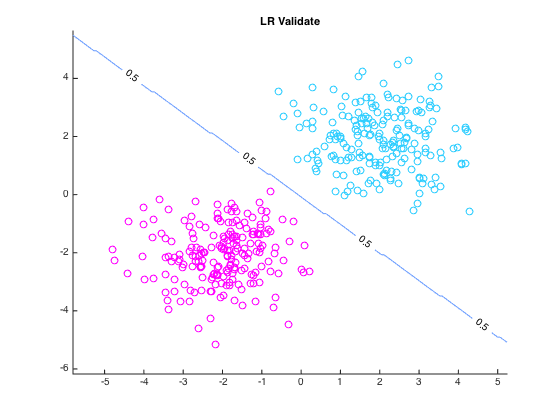
\includegraphics[width=\linewidth]{figures/sd1v2.png}
  \caption{\texttt{stdev = 1}}\label{fig:gradDifQ}
\endminipage\hfill
\minipage{0.25\textwidth}
  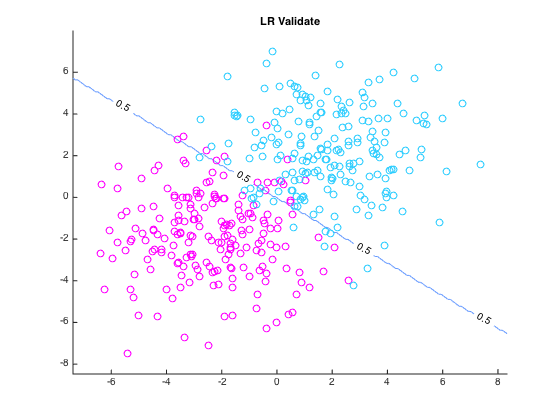
\includegraphics[width=\linewidth]{figures/sd2v20.png}
  \caption{\texttt{stdev = 2}}\label{fig:gradDifN}
\endminipage\hfill
\minipage{0.25\textwidth}
  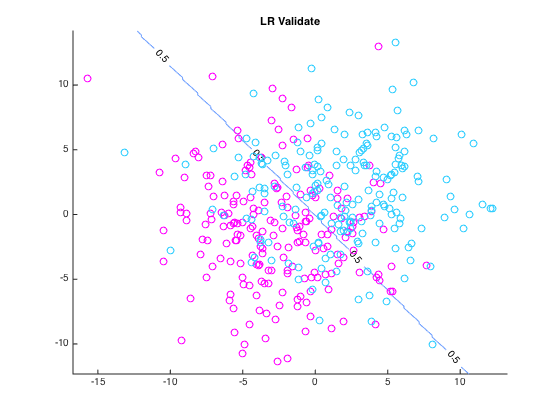
\includegraphics[width=\linewidth]{figures/sd4v20.png}
  \caption{\texttt{stdev = 4}}\label{fig:gradDifS}
\endminipage\hfill
\minipage{0.25\textwidth}
  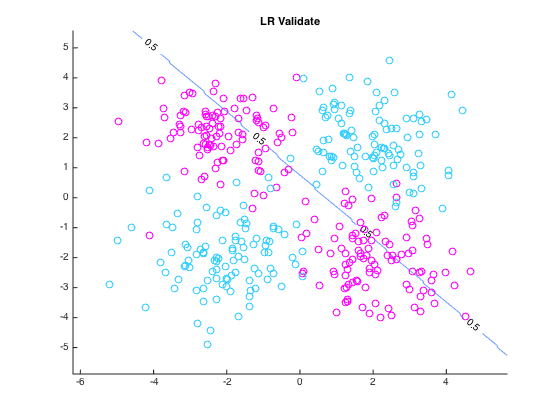
\includegraphics[width=\linewidth]{figures/sdnv20.png}
  \caption{\texttt{unseparable}}\label{fig:gradDifS}
\endminipage

\end{figure}

Figures 1-4 show the training data, and figures 5-8 show the validation data for $\lambda = 0$. The predictor is reasonably effective and seems to seek to minimize the loss. When we increase $\lambda$, however, we instead increase the loss as we try to minimize the $\lambda w^\intercal w$ term in the error function. This means that the model is more inaccurate in this case, which is because with two parameters, $w$ wasn't likely going to overfit to the data anyways. But note that the effect is not too large, even for larger $\lambda$ ($\lambda = 40$) - our main goal is still to minimize the total error.




\section{Support Vector Machines}
\subsection{Overview and Formulation}
Support Vector Machines are a machine-learning technique that is used to classify binary sets of data. We define $\theta$ as the normal to the decision hyperplane, and classify data points by $\sign (\theta^\intercal x + \theta_0)$. In order to train the classifier, we initially set up the minimization problem (known as \textbf{Hard-SVM}):

\begin{equation}
\max_{\theta, \theta_0} \dfrac{1}{||\theta||} \min_{1 \le i \le n} y^{(i)} (\theta^\intercal x^{(i)} + \theta_0)
\end{equation}

However, we cannot satisfy this minimization if the training set is not linearly separable. Therefore, we add a ``slack variable'' to each constraint, which is a measure of the ``wrongness'' of the decision boundary when classifying that point. We call these slack variables $\xi_i$. We then desire to minimize
\begin{align}
\min_{\theta, \theta_0, \xi} \dfrac{\lambda}{2} ||\theta||^2 + \dfrac{1}{n} \sum_{i=1}^{n} \xi_{i} &, \\
s.t. \hspace{.75em} y^{(i)}(\theta^\intercal x^{(i)} + \theta_0) \ge 1 - \xi_i &, \\
\xi_i \ge 0, i \in n &
\end{align}

However, we find it more computationally efficient to solve the dual form of the \textbf{Soft-SVM}:
\begin{align}
\max_{\alpha \in \mathbb{R}^n} \left[ \sum_{i=1}^n \alpha_i - \dfrac{1}{2} \sum_{i=1}^n \sum_{j=1}^n \alpha_i \alpha_j y^{(i)} y^{(j)} (x^{(i)})^\intercal x^{(j)}\right] & \\
s.t. \hspace{.75em} 0 \le \alpha_i \le C & \\
\sum_i \alpha_i y^{(i)} = 0 &
\end{align}

To provide some intuition: $\alpha_i$ is the weight of each training point on the final decision boundary. It is 0 for all $x^{(i)}$ that are farther from the decision boundary than the margin, so that only the ``important'' $x^{(i)}$ are ``support vectors''. $C$ is the maximum value of $\alpha$, and determines the size of the margin. In particular, for small $C$, the margin is very large, and vice versa. To return from $\alpha$ to the more familiar $\theta$ and $\theta_0$, we plug in:
\begin{align}
\theta &= \sum_{i=1}^n \alpha_i y^{(i)} x^{(i)} \\
\theta_0 &= \dfrac{1}{\mathcal{M}} \left[ \sum_{j \in \mathcal{M}} \left( y^{(j)} - \sum_{i \in \mathcal{S}} \alpha_i y^{(i)} (x^{(j)})^\intercal x^{(i)} \right) \right]
\end{align}

Where $\mathcal{M} = \{ i : 0 < \alpha_i < C \}$ and $\mathcal{S} = \{ i : 0 < \alpha_i \}$.

For example, given the data $X = [1, 2;\ 2, 2;\ 0, 0;\ -2, 3], Y = [1;\ 1;\ -1;\ -1]$, we generate the following objective function and constraints (taking the opportunity to insert a kernel function, $K$):

\begin{equation}
\max_{\alpha \in \mathbb{R}^n} \left[\sum_{i=1}^n \alpha_i - \dfrac{1}{2} \sum_{i=1}^n \sum_{j=1}^n \alpha_i \alpha_j y^{(i)} y^{(j)} (x^{(i)})^\intercal x^{(j)} \right] \\
\Leftrightarrow \min_{\alpha \in \mathbb{R}^n}\left[\dfrac{1}{2} \alpha^\intercal H \alpha + f^\intercal \alpha\right]
\end{equation}
\begin{align}
H_{i,j} =&\ y^{(i)} y^{(j)} K(x^{(i)},x^{(j)}) \\
f =&\ [-1\ -1\ \ldots\ -1]\ \text{(of length $n$)} \\
&\ s.t. \hspace{.75em} Y^\intercal \alpha = 0 \\
&\ s.t. \hspace{.75em} 0 \le \alpha_i \le C, \forall i \in n
\end{align}

\subsection{Testing Implementation}

Applying our implementation of the soft-SVM to the 4 datasets from part 1, setting $C = 1$, we obtain the classifiers in \ref{fig:stdev1} - \ref{fig:nonsep}. We note that the classifiers are reasonable for the three separable data sets, and that the margin grows as the standard deviation of the test sets increases. This makes sense - we are less sure about the classification for these, so the margin grows. Our validation errors were 0.0822, 68.67, 227.0, and 404.7, respectively. The training errors were 1.16, 88.56, 240.9, and 396.6, respectively. Again, these errors are logical and match what we expect - as the data becomes less easily separable, the error increases.

\begin{center}
\begin{figure}[!htb]
\minipage{0.48\textwidth}
  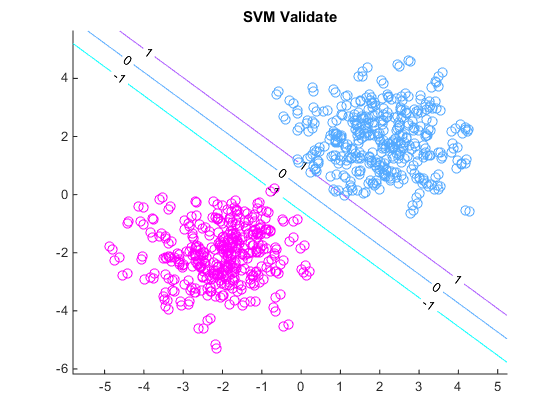
\includegraphics[width=\linewidth]{figures/stdev1.png}
  \caption{\texttt{stdev = 1}}\label{fig:stdev1}
\endminipage\hfill
\minipage{0.48\textwidth}
  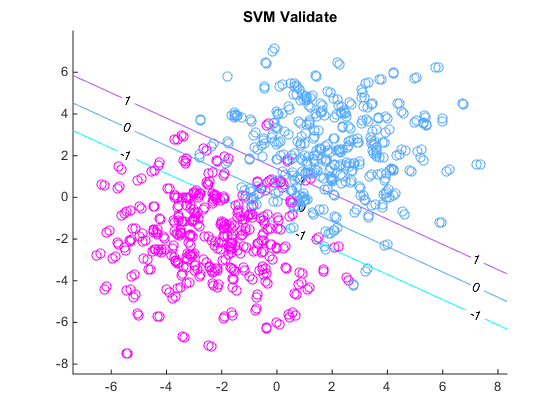
\includegraphics[width=\linewidth]{figures/stdev2.png}
  \caption{\texttt{stdev = 2}}
\endminipage
\end{figure}
\begin{figure}[!htb]
\minipage{0.48\textwidth}
  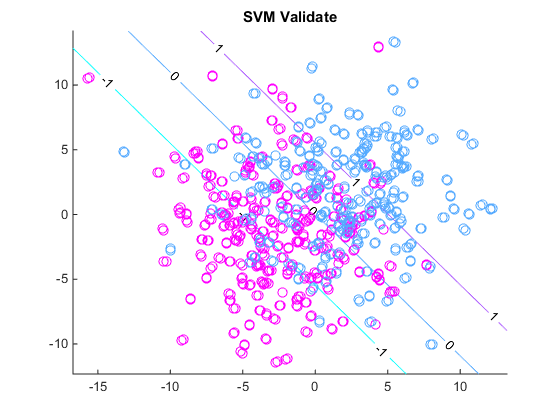
\includegraphics[width=\linewidth]{figures/stdev4.png}
  \caption{\texttt{stdev = 4}}
\endminipage\hfill
\minipage{0.48\textwidth}
  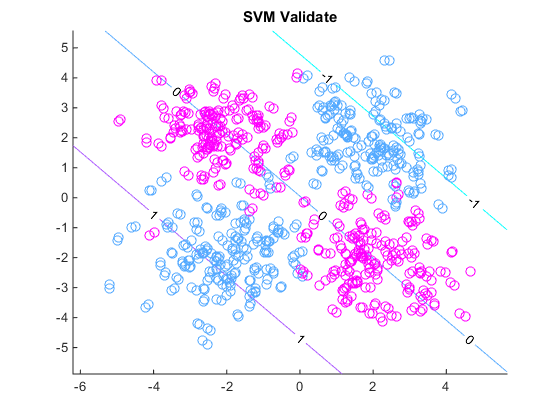
\includegraphics[width=\linewidth]{figures/nonsep.png}
  \caption{\texttt{unseparable}}\label{fig:nonsep}
\endminipage
\end{figure}
\end{center}

\subsection{Kernel Extension}
As was briefly mentioned in 2.1, we can easily insert a kernel function into the dual form of the SVM. In this particular case, we choose to insert the Gaussian Radial Basis Function (RBF):

\begin{equation}
K(x_1,x_2) = \exp\left( -\dfrac{||x_1-x_2||^2}{2\sigma^2} \right)
\end{equation}

This is particularly useful, because instead of looking at the dot product of $x_1$ and $x_2$, we instead may examine the distance between them, allowing us to find radially clustered groups. In this formulation, $\sigma$ is a scalar, and so all dimensions must be normalized with respect to their std deviation in order to obtain meaningful results. Alternative formulations exist that have vector $\sigma$ to account for variances in std deviation. Applying the RBF kernel to the \texttt{nonsep} dataset, setting $\sigma = 1$ and varying $C$, we obtain the classifiers in figures \ref{fig:c01} - \ref{fig:c100}.

\begin{center}
\begin{figure}[!htb]
\minipage{0.32\textwidth}
  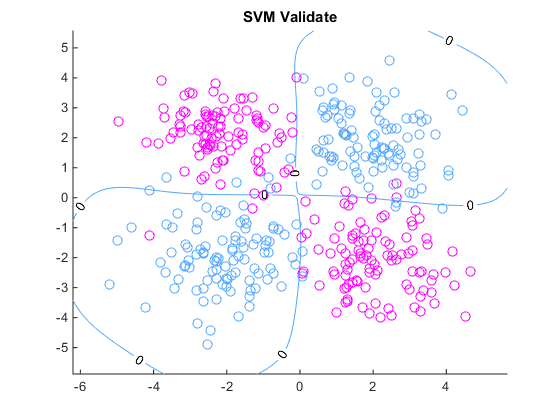
\includegraphics[width=\linewidth]{figures/C,01sigma1.png}
  \caption{$C = 0.01, \sigma = 1$}\label{fig:c01}
\endminipage\hfill
\minipage{0.32\textwidth}
  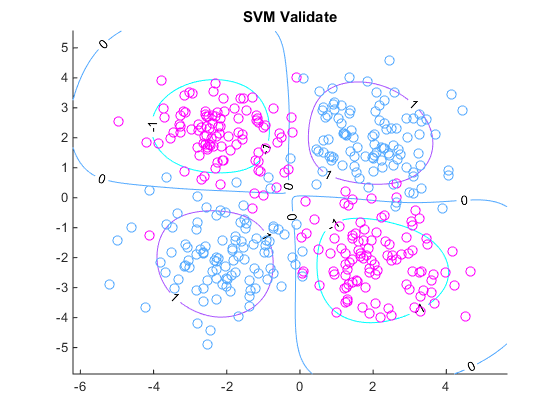
\includegraphics[width=\linewidth]{figures/C,1sigma1.png}
  \caption{$C = 0.1, \sigma = 1$}
\endminipage\hfill
\minipage{0.32\textwidth}
  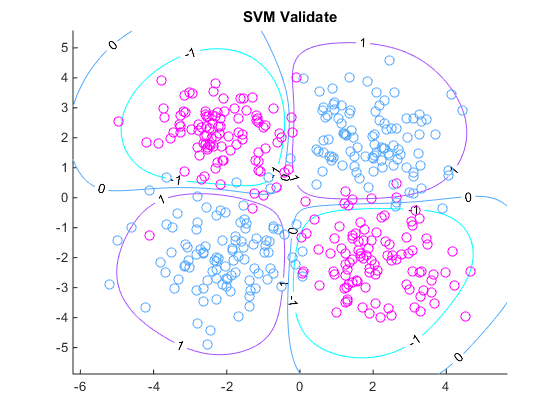
\includegraphics[width=\linewidth]{figures/C1sigma1.png}
  \caption{$C = 1, \sigma = 1$}
\endminipage
\end{figure}
\begin{figure}[!htb]
\hspace{.16\textwidth}
\minipage{0.32\textwidth}
  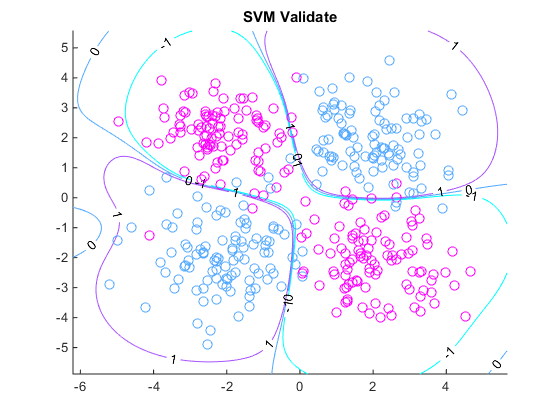
\includegraphics[width=\linewidth]{figures/C10sigma1.png}
  \caption{$C = 10, \sigma = 1$}
\endminipage
\minipage{0.32\textwidth}
  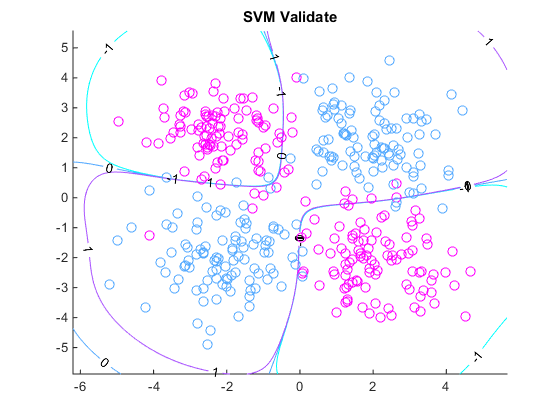
\includegraphics[width=\linewidth]{figures/C100sigma1.png}
  \caption{$C = 100, \sigma = 1$}\label{fig:c100}
\endminipage
\end{figure}
\end{center}

We also note that as $C$ increases, the number of boundary points decreases. Thus, the number of support vectors decrease. For the nonseparable example, for $C = (.01, .1, 1, 10, 100)$, we see that $\mathcal{M} = (400, 324, 133, 68, 59)$. Varying $\sigma$, we notice that the ``clusters'' the classifier finds are composed of many smaller Gaussians for small $\sigma$ and composed of fewer larger Gaussians for larger $\sigma$. Basically, the size of the ``clumps'' the classifier looks for proportional to $\sigma$.

As per the usual procedure we used in regression on the approximately equivalent $\lambda$, to select the correct $C$ we first compute $\alpha$ for various values of $C$ using a training set, then determine the validation error using a validation set. We select the $C$ which produces the lowest validation error in order to maximize the generality of our solution.
\section{Titanic Data}

\subsection{LR}
As an application of our work from previous sections, we can apply both logistic regression and SVMs to a real dataset, namely, separating passengers on the Titanic into survivors and those who were lost at sea. Unlike the previous data, this dataset has 11 parameter columns, each corresponding to some feature of the passengers that we are modeling. Before we do anything, however, we ensure that we are working with a reasonable dataset by scaling the features to have $\mu = 0$ and $\sigma^2 = 1$. This gives us the parameters in Table 2. From this data, we can see that there is a noticeable relationship between sex and survival; we can plot sex and age to see that there is indeed a correlation in figure \ref{sexagelr}.

\begin{minipage}{\textwidth}
\begin{minipage}[b]{.4\textwidth}
\centering
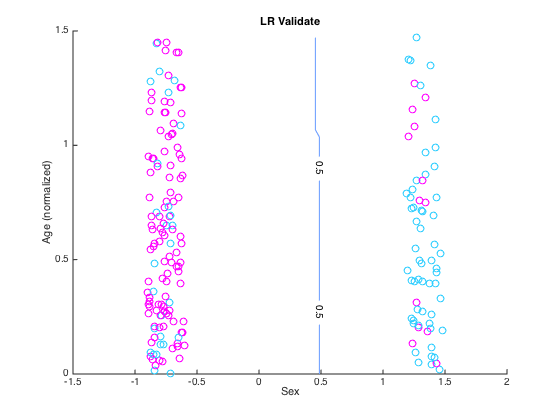
\includegraphics[width=\linewidth]{figures/titanic45.png}
\captionof{figure}{Decision boundary considering only age and sex}\label{sexagelr}
\end{minipage}
\hfill
\begin{minipage}[b]{.59\textwidth}
\centering
\begin{tabular}{rlc}
Column & Meaning                           & $\theta_i$\\ \hline
1      & Passenger Class 1                 & 0.5843  \\
2      & Passenger Class 2                 & 0.5169  \\
3      & Passenger Class 3                 & -0.2008 \\
4      & Sex                               & 1.2356    \\
5      & Age                               & -0.3297 \\
6      & Number of Siblings/Spouses Aboard & -0.1402 \\
7      & Number of Parents/Children Aboard & 0.1596  \\
8      & Passenger Fare                    & 0.1206   \\
9      & Embark from Southampton           & -0.0816 \\
10     & Embark from Cherbourg             & 0.1178  \\
11     & Embark from Queenstown            & -0.0349  \\
\end{tabular}
\captionof{table}{$\theta_i$ for $\lambda = 1$.}

\end{minipage}

\end{minipage}

\subsection{SVM}
Now, we apply the SVM to the Titanic dataset. We apply the standard method to select $C$ (ie, calculate the loss on the validation set for the classifiers trained with the training set for various values of $C$.) Applying this method, we get $C = 0.1$, which leads to a validation error of 81.1067. The classifier this creates, using a linear kernel, is summarized in Table 3. We can clearly see from $\theta_i$ that sex is by far the most important factor towards determining $y$. Plotting in Figure 23, for example, sex on the x-axis and age on the y-axis, as well as the $\theta$ generated when considering just these two factors, we see that the examples are split fairly well by sex, but age is well-mixed. In the plot, we add a scattering factor of some random number in $[-.15,.15]$ to the plotted points ($\theta$ is trained on the points before the scattering factor).

\begin{minipage}{\textwidth}
\begin{minipage}[b]{.4\textwidth}
\centering
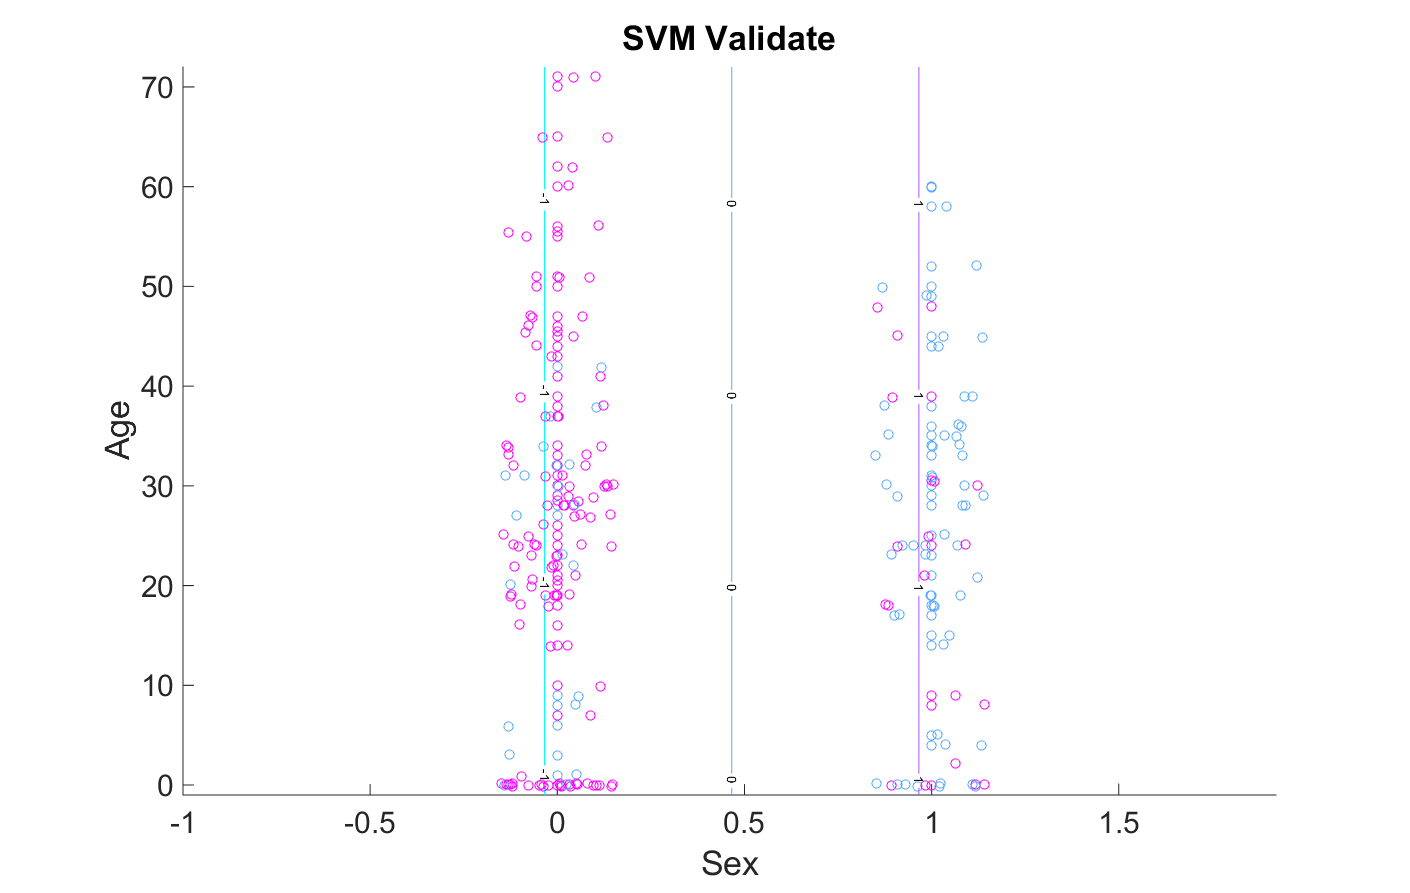
\includegraphics[width=\linewidth]{figures/sex_age_validate.png}
\captionof{figure}{Decision boundary considering only age and sex}\label{sexagelr}
\end{minipage}
\hfill
\begin{minipage}[b]{.59\textwidth}
\centering
\begin{tabular}{rlc}
Column & Meaning                           & $\theta_i$\\ \hline
1      & Passenger Class 1                 & 2.02e-04  \\
2      & Passenger Class 2                 & 3.87e-04  \\
3      & Passenger Class 3                 & -5.89e-04 \\
4      & Sex                               & 2.00      \\
5      & Age                               & -1.10e-05 \\
6      & Number of Siblings/Spouses Aboard & -5.64e-05 \\
7      & Number of Parents/Children Aboard & 3.10e-04  \\
8      & Passenger Fare                    & 2.77e-06  \\
9      & Embark from Southampton           & -3.20e-04 \\
10     & Embark from Cherbourg             & 1.68e-04  \\
11     & Embark from Queenstown            & 1.52e-04  \\
\end{tabular}
\captionof{table}{$\theta_i$ for $C = .1$.}

\end{minipage}

\end{minipage}

Overall, our final testing error is 81.1. The particular values of $\theta$ could be made more reasonable by normalizing the data sets based on the mean and standard deviation, but the overall trend that sex is the defining factor remains the same.

\subsection{Comparing and Contrasting LR and SVM}
Comparing the results from LR and SVM, we see that they are very similar. They both report the sex as the most important factor when determining $y$, by a large margin. Feature scaling before applying LR is critical in order to avoid convergence towards infinity, but SVM can converge before feature scaling, though it would benefit from feature scaling, since not all of the features have the same scale. However, since many of them are binary, it doesn't make much difference in this particular case.
\end{document}













